% xelatex
\documentclass{article}
\usepackage[czech]{babel}
\usepackage{polyglossia}
\setmainlanguage{czech}

\usepackage{graphicx}
\usepackage{url}

\usepackage{dirtree} %directory tree visualisation
\usepackage{graphicx}
\usepackage{listings}
\usepackage{minted}
\usepackage{multirow}
\renewcommand{\listingscaption}{Výpis kódu}
\renewcommand{\listoflistingscaption}{Seznam výpisů kódu}

\title{Řešení problému vážené splnitelnosti booleovské formule pokročilou iterativní metodou} %doplňte název bakalářské práce
\author{\small Mikhail Karimov}
\date{\small Fakulta informačních technologií Českého vysokého učení technického v Praze\\ \url{karimmik@fit.cvut.cz}} %doplňte svůj email


\begin{document}

\maketitle

% \usepackage{amsmath} %advanced maths
% \usepackage{amssymb} %additional math symbols

\section{Zadaní}

Dána Booleova formule \(F\) o \(n\) proměnných, \(X=(x_1, x_2, ... , x_n)\) v konjunktivní normální formě (CNF). Dále jsou dány celočíselné kladné váhy těchto \(n\) proměnných \(W=(w_1, w_2, ... , w_n)\). Nalezněte přiřazení \(Y=(y_1, y_2, ... , y_n)\) proměnných \(x_1, x_2, ... , x_n\), takové, že \(F(Y)=1\) a součet \(S\) vah proměnných nastavených do 1 je maximální. 

Omezte se na vážený 3-SAT problém, kde každá klauzule má právě 3 proměnné. Složitost problému je stejná, implementace a klasifikace instancí jsou jednodušší

\subsection{Charakterizace problému}

Jde o konstruktivní problém.

\begin{itemize}
\item Vstupní proměnné v daném případe je Booleova formule \(F\) o \(n\) proměnných a váhy jednotlivých proměnných \(W\).
\item Výstupní proměnná je konfigurace \(Y=(y_1, y_2, ..., y_n)\) s nejvýší hodnotou optimalizačního kriteria a taková, že \(F(Y)=1\).
\item Konfigurace problému je \(Y=(y_1, y_2, ..., y_n)\), kde každé proměnné Booleově formule přiřazeno bud \(1\) nebo \(0\).
\item Omezení je hodnota Booleově formule po přiřazení konfigurace.
\item Optimalizační kriterium je součet vah proměnných nastavených do 1.
\end{itemize}

\newpage
\section{Implementace}

Na řešení teto úlohy jsem zvolil a implementoval algoritmus Simulované Evoluce(dál jen SE. Moje implementace SE obsahuje fází:
\begin{itemize}
\item Generace počáteční populace, kdy se náhodné vygenerují inicializační konfiguraci.
\item Generační cyklus:
	\begin{itemize}
	\item Selekce
	\item Křížení
	\item Mutace
	\item Náhrada populace
	\end{itemize}
\end{itemize}

Implementace je v jazyku Python. S využitím principů OOP:
\begin{itemize}
\item Třída \(Solution\) reprezentuje konfigurace, s nastavitelnou cenou konfigurace, má metody na mutace a křížení.
\item Třída \(SAT_Instance\) je jednoduchá implementace Booleově formule, která umí ohodnotit řešení a přečíst formule ze souboru. Neumí hledat řešení.
\item Třída \(SAT_SE_Instance\) je implementace SE algoritmu a v ní se prochází hlavní část výpočtu řešení.
\item Soubor \(SAT_File\)\\ obsahuje funkce na čtení optimálního řešení ze souboru.
\item Pomocí tříd \(Jupyter_Graph\) a \(Jupyter_Scatter\) lze sestrojit vhodný vstup pro Pyplot na vizualizací.
\end{itemize}


\subsection{Kódovaní řešení}

Konfigurace řešení se kóduje do binárních řetězců. Na implementace použil jsem jednotlivou třídu \(Solution\), která se stará o chránění binárního konfiguračního vektoru a jeho hodnoty-váhy.


\subsection{Selekce}

Na selekce použil jsem turnajový mechanismus, kde se z populací zvolí náhodně několik členu a z nich najdu nejlepšího, kterého přidám do seznamu potenciálních rodičů. Turnaj se opakuje \(n\)-krát(\(n\) je počet prvků populací) dokud nenaplní seznam potenciálních rodičů. Selekční tlak v turnaji se řídí změnou kapacity turnaje. Počet nástupců řídím v závislostí na poměr střední hodnoty a směrodatné odchylky předchozí generace. Minimální kapacita je 2.

\begin{listing}[H]
\begin{minted}[mathescape,
			   fontsize=\small,
               linenos,
               numbersep=5pt,
               gobble=2,
               frame=lines,
               framesep=2mm]{python}
        
...        
    if stredni_hodnota != 0 and
    abs(smer_odchyl/stredni_hodnota) > nastavitelny_parametr and
    kapacita_turnaje > 2:
        kapacita_turnaje = floor(kapacita_turnaje * 0.9)
...
               
\end{minted}
\caption{Implementace řízení turnajové kapacity}
\label{implementace:tournament}
\end{listing}


\subsection{Křížení}   

Křížení provádím uniformním způsobem(zjistím ze kterého rodiče do kterého potomka nakopíruji genetické informace pomocí náhodné vygenerovaného vektoru). Rodiče volím náhodné ze seznamu potenciálních rodičů, a z každého kříženi se vytvoří dva potomci, které zapíšu do populace.

\begin{figure}[H]
    \centering
    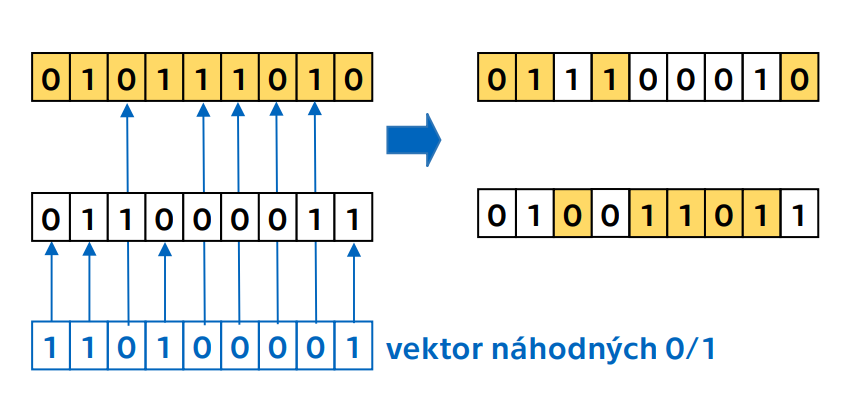
\includegraphics[width=1\textwidth]{Screenshot_1228}
    \caption{Základní myšlenka uniformního křížení\cite{recomb_uni}}
    \label{fig:recomb_uniform}
\end{figure}

\subsection{Mutace}   

Mutace provedu tak, že náhodné změním jednu hodnotu v konfiguračním vektoru jednoho náhodného člena populace.

\subsection{Náhrada populace}

Z populace výběru do nové generací \(n\) nejlepších jedinců podle hodnoty.

\newpage
\subsection{Omezující váhová podmínka}

Základní metoda, kterou jsem použil na zajištění omezující podmínky v SE je Relaxace. V implementaci je to tak, že jedince se porovnávají podle váhy řešení(atribut \(value\) v objektu \(Solution\)), jen že pokud není řešením, tak hodnotu \(value\) nastavím na:

\[ -1 * \frac{pocet\_klauzuli - pocet\_splnenych\_klauzuli}{pocet\_klauzuli}\]

Protože hodnota ceny je záporná tak je jedinec, který není řešením, má menší cenu než jakékoliv řešení. A ve množině neřešení ze dvou prvků jsem schopen porovnat který je další od řešení.\\

V podstatě pří nastavení relaxace by mně zajímal "směr" relaxace: hodnota konfigurace by měla se \uv{vylepšit} co nejvíc po změně hodnoty na \uv{správnou} u \uv{správného} prvku konfiguračního vektoru. Nicméně nepodařilo se mně najít za daný čas takovou relaxace. Moje relaxace se nebere do úvahy váhy jednotlivých proměnných formule, ale jen posouvá algoritmus do nějakého řešení.

To, že hodnota neřešení muže se nabývat [-1, 0) jsem využil k návrhu vlastního operátoru SE.

\subsection{Vlastní operator SE}

Protože jsem omezil čeho se muže nabývat hodnota konfigurace, která není řešením. Mohl by jsem to využit k ošetřování nejhorších možných konfigurací.

\begin{listing}[H]
\begin{minted}[mathescape,
			   fontsize=\small,
               linenos,
               numbersep=5pt,
               gobble=2,
               frame=lines,
               framesep=2mm]{python}
        
...        
       for index, konfigurace in enumerate(populace):
            if konfigurace.hodnota < -0.8:
                populace[index] = nová_náhodná_konfigurace
                populace[index].nastav_hodnotu(...)

...
               
\end{minted}
\caption{Implementace náhrady jedinců populace s nejhorší hodnotou}
\label{implementace:tournament}
\end{listing}

Například, než by jsem dlouho bloudil od konfigurace, která není řešením a je velmi daleko od řešení, by mohl takovou konfigurace nahradit nějakým novým náhodným konfiguračním vektorem, který by s dostatečnou pravděpodobnosti měl vetší hodnotu.

Podle kódu \ref{implementace:tournament} nahradím 20\% nejhorších možných konfigurací, které není řešením. Budu mít šance minimálně 80\% dostat nějakou lepší konfiguraci.

\subsection{Ukončovací podmínka}

Program se běží dokud směrodatná odchylka prvků z populace se nerovná nule. Jinými slovy program se zastaví když celá generace se skládá ze stejných prvků.        

\newpage
\section{Experiment}
\subsection{Podmínky a prostředí}
Na testování implementace použil jsem sbírku instancí ze stránek předmětu NI-KOP.

Moje PC sestava je:
\begin{itemize}
\item Intel Core I5 8400 2.8 GHz
\item 16 GB RAM 2666 MHz
\item Windows 10 Home
\end{itemize}

Bechem měření výsledků na počítače běželi další programy(webový prohlížeč).

\subsection{Parametry implementace SE}

Celkový seznam nastavitelných parametru je:
\begin{itemize}
\item \(population\_multiple\): multiplikátor velikosti populace.
\item \(recombination\_multiple\): multiplikátor počtu kříženi. Pozor: výsledkem křížení je dva prvky.
\item \(tournament\_size\_multiple\): multiplikátor počáteční velikosti turnaje. Velikost turnaje se řídí adaptivně v době běhu programu.
\item \(pop\_reborn\): jestli má se zapnout vlastní operator.
\end{itemize}

Implementace je cílena řešit problémy, kde počet proměnných a klauzí ve formule se může lišit. Proto asi vhodné se zaměřit na zjištění ne konkretních hodnot parametrů ale jejích poměru k instančním proměnným.\\   

Počet kříženi podle by měl spíš role podpůrného nebo pokročilejšího parametrů, který se nemění chování programu tak moc než v souvislostí s parametrem velikosti turnaje:
\begin{itemize}
\item Když seznám potenciálních rodičů obsahuje moc duplicit, tak je s růstem počtu křížení se roste pravděpodobnost, že do kříženi se dostanou dvě duplicity a výsledkem je duplicita konfigurace z populace. Což vede k degenerací populace.
\item S velkým počtu unikátních jedinců v seznamu potenciálních rodičů pravděnepodobnější dokážu vygenerovat víc nových prvků.
\end{itemize}
Seznám potenciálních rodičů se závislý na velikost turnaje. Proto parametr \(recombination\_multiple\) budu zkoumat v souvislostí s tou myšlenkou.

\subsection{Zkoumaní chování algoritmu v závislosti na hodnoty parametrů}

Cílem teto častí je zjistit jak se závisí chování programu na změnu vstupních parametrů. Pro účely experimentu u náhodného generátoru je nastaveno \(seed\).

\subsubsection{Velikost populace}

Jediné na čemž je závislá velikost populace je počet proměnných v Booleově formule. Měl jsem nápad že by mohla ta velikost se záviset i na počet klauzí, ale ty klauzi spíš jen omezují počet platných konfigurací. Velikost konfigurace nebo konfiguračního řetězce se závislá jen na počet proměnných.

Počáteční velikost turnaje a počet křížení nastavuji v zavilostí na velikost populace pomocí nastavitelných multiplikátorů. Proto parametry \(recombination\_multiple\) a \(tournament\_size\_multiple\) jsou závislé na multiplikátor \(population\_multiple\), kterým nastavuji velikost populace.

\begin{figure}[H]
    \centering
    \includegraphics[width=0.8\textwidth]{screenshot_1280}
    \caption{Vývoj nejlepší ceny v populace. \(population\_multiple = 1\)}
    \label{fig:se_pm1}
\end{figure}

Podle obrázku \ref{fig:se_pm1} se vypadá, že SE má hlad na jedince pří \(population\_multiple =1\):
\begin{itemize}
\item Nepodařilo se u žádného spuštění pří inicializací počáteční populace vygenerovat ani jedné platné řešení.
\item Jsou tam spuštění, které udusily se bez zdrojů ke křížení: spuštění 8 a 6 vůbec nenašly platnou konfiguraci.
\item Jsou tam zároveň i ty, které našly, ale s docela malou hodnou.
\item Hlavně že půlka z tech, které našly nějaké řešení, se skočila do toho a už neměnila se.
\end{itemize}

\begin{figure}[H]
    \centering
    \includegraphics[width=1\textwidth]{screenshot_1281}
    \caption{Vývoj nejlepší ceny v populace. \(population\_multiple = 1.5\)}
    \label{fig:se_pm15}
\end{figure}

Podle mně pří \(population\_multiple=1.5\) na obrázku \ref{fig:se_pm15} chovaní algoritmu příliš neliší od předchozího nastavení. Ano, povedlo se vygenerovat platné řešení v počáteční populace, ale grafy pořad hodně skoků nemají. Rychlá degenerace populace.

\begin{figure}[H]
    \centering
    \includegraphics[width=1\textwidth]{screenshot_1283}
    \caption{Vývoj nejlepší ceny v populace. \(population\_multiple = 2\)}
    \label{fig:se_pm2}
\end{figure}

K výsledkům \(population\_multiple = 2\), které jsou na obrázku \ref{fig:se_pm2}, asi nemůžu říct nic zajímavého: vypadají se rozumně.\\

Na následující stránce jsou obrázky \ref{fig:se_pm3} a \ref{fig:se_pm5}, které se reprezentují chování algoritmu pří nastavení parametru \(population\_multiple=3\) (resp. \(population\_multiple=5\)). Grafy ceny se mají víc a víc skoku se zvýšením velikosti populace. Už tam víc řešení(i docela dobrých), které podařilo vygenerovat v počáteční populace. Samozřejmé že se zvýšením velikosti populace se roste pravděpodobnost dostat řešení až na začátku.\\

Řekl bych že na účel testování ostatních parametrů hodnota \(population\_multiple=2\) je postačující.

\newpage
\begin{figure}[H]
    \centering
    \includegraphics[width=1\textwidth]{screenshot_1284}
    \caption{Vývoj nejlepší ceny v populace. \(population\_multiple = 3\)}
    \label{fig:se_pm3}
\end{figure}

\begin{figure}[H]
    \centering
    \includegraphics[width=1\textwidth]{screenshot_1285}
    \caption{Vývoj nejlepší ceny v populace. \(population\_multiple = 5\)}
    \label{fig:se_pm5}
\end{figure}
\newpage

\subsubsection{Počet křížení a počáteční velikost populace}

Podle obrázků \ref{fig:se_4110}, \ref{fig:se_12110}, \ref{fig:se_415}, \ref{fig:se_1215}:
\begin{itemize}
\item Pří nízkých hodnotách multiplikátorů počtu křížení a počáteční velikosti turnaje žádné spuštění nedosáhlo optimální ceny.
\item Pří nízkých hodnotách multiplikátorů počtu křížení a počáteční velikosti turnaje algoritmus potřebuje víc generací a stálé má horší výsledky než u dostatečně velkých hodnot.
\end{itemize}

Pointa je asi v principu křížení. Je množina všech variant výsledků křížení dvou konfigurací a v tě množině prvky mají různou cenu. S velkým počtem kříženi je vetší pravděpodobnost z množiny potenciálních potomků dostat dobrý výsledek. Proto s velkým počtem křížení zkusím dat rodičům šance vygenerovat lepšího potomka i když rodiče není řešením.

S velkou konkurencí pří velkém turnaje pravděpodobné budu dostávat víc duplicit. Ze dvou duplicit nedokážu vygenerovat žádný nový prvek a proto se množina dětí bude se sestavovat ze 'dvojčat'. Pokud se náhodné najdu dobrou konfiguraci, tak se začnou ti dvojčata mně vytlačovat všechny konfigurace s horší cenou, i když obsahují nějakou dobrou část genomu: degenerace populace.\\

Nicméně podle obrázků \ref{fig:se_4110}, \ref{fig:se_12110}, \ref{fig:se_415}, \ref{fig:se_1215} jsem zvolil nastavení hodnot parametrů: \(recombination\_multiple=4\), \(tournament\_size\_multiple=1/10\).

\begin{figure}[H]
    \centering
    \includegraphics[width=1\textwidth]{screenshot_1286}
    \caption{Vývoj nejlepší ceny v populace.\newline \(recombination\_multiple=4\),\(tournament\_size\_multiple=1/10\)}
    \label{fig:se_4110}
\end{figure}

\begin{figure}[H]
    \centering
    \includegraphics[width=1\textwidth]{screenshot_1287}
    \caption{Vývoj nejlepší ceny v populace.\newline \(recombination\_multiple=1/2\),\(tournament\_size\_multiple=1/10\)}
    \label{fig:se_12110}
\end{figure}


\begin{figure}[H]
    \centering
    \includegraphics[width=1\textwidth]{screenshot_1291}
    \caption{Vývoj nejlepší ceny v populace.\newline \(recombination\_multiple=4\),\(tournament\_size\_multiple=1/5\)}
    \label{fig:se_415}
\end{figure}

\begin{figure}[H]
    \centering
    \includegraphics[width=1\textwidth]{screenshot_1292}
    \caption{Vývoj nejlepší ceny v populace.\newline \(recombination\_multiple=1/2\),\(tournament\_size\_multiple=1/5\)}
    \label{fig:se_1215}
\end{figure}

\subsection{Závěr sekce nastavení parametrů}
Zvetšení velikosti populace má positivní vliv na chování algoritmu. Jinak je otázka efektivity jestli se stojí zvětšovat tu velikost do nějakých extrémních veličin. Doporučím držet se alespoň dvojnásobku počtu proměnných z Booleově formule.

Velký počet kříženi má positivní vliv na evoluce populace pokud nekřížím duplicity.

Otázka, jestli šlo by prozkoumat víc hodnot parametrů, je předmětem další diskuze. Myslím že samozřejmě by šlo prozkoumat hodnoty i do desetinných míst, ale spíš by soustředil na otázku navrchu a vývoje optimálnější implementace. Práce s heuristikou je skoro vždy otázka stojí li vylepšení výsledků na několik procent, pokud za to potřebuji dávat víc času, peněz a sil.

Lze tady i zároveň vidět iterativní silu pří různém nastavení parametrů.

\newpage

\section{Hromadné testování na instancích}

Cílem teto častí je prokázat a ohodnotit zavilost algoritmu na vstupní proměnný problému a měření času.

\subsection{Hromadné měření času}

Na účely testování jsem používal vždy prvních 100 instancí z resp. sbírky, ke kterým mám optimální odpověď - konfigurační vektor s nejvyšší dosažitelnou cenou řešení. Připomínám, že pro účely testování RNG má nastavený \(seed\) a že Garbage Collector se vyprázdní před každým spuštěním. Počet proměnných Booleově formule u instancí je vždy 20. U sady instancí A počet klauzí je 88, jinak je 78.\\

Na libovolném obrázku z \ref{fig:se_t1},\ref{fig:se_t2},\ref{fig:se_t3} lze pozorovat stupňové seskupovaní výsledků měření, které by mělo odpovídat počtu generací u jednotlivého spuštění. Lze vidět, že ve většině případů výpočet se běžel v intervalu (250,300) ms nezávisle na sbírku instancí. Maximální dobu běhu by ohodnotil jako 500 ms, a případy, ve kterých doba běhu je vetší, bych možné považoval za výjimku, způsobenou Garbage Collector'em nebo programem bežícím na pozadí.

\begin{figure}[H]
    \centering
    \includegraphics[width=1.2\textwidth]{screenshot_1294}
    \caption{Vizualizace výsledků měření času u sad instancí M a N}
    \label{fig:se_t1}
\end{figure}


\begin{figure}[H]
    \centering
    \includegraphics[width=1.2\textwidth]{screenshot_1293}
    \caption{Vizualizace výsledků měření času u sad instancí R a Q}
    \label{fig:se_t2}
\end{figure}

\begin{figure}[H]
    \centering
    \includegraphics[width=1.2\textwidth]{screenshot_1295}
    \caption{Vizualizace výsledků měření času u sady instancí A}
    \label{fig:se_t3}
\end{figure}

\newpage
\subsection{Hromadné měření relativně chyby}
\begin{table}[H]
\begin{tabular}{|l|l|l|}
\hline
\textbf{Sada instancí} & \textbf{Střední rel. chyba u instance} & \textbf{Rel. chyba algoritmu na sadě instancí} \\ \hline
\textbf{N} & 0,0242 & 0,1720 \\ \hline
\textbf{M} & 0,0202 & 0,1581 \\ \hline
\textbf{R} & 0,1136 & 0,3920 \\ \hline
\textbf{Q} & 0,1326 & 0,4553 \\ \hline
\textbf{A} & 0,3070 & 1,0000 \\ \hline
\end{tabular}
\caption{Výsledků měření rel. chyby}
\label{fig:se_errors}
\end{table}

Je mi líto zkoumat výsledky měření chyby algoritmu. U sady instancí A je poznámka že v teto sade kvůli malému počtu správných řešení algoritmus má velkou šance najít správné řešení. U sad N a M naopak je poznámka, že by měla tam relativní chyba být dost velká kvůli tomu že je tam víc řešení.

Já mám zcela naopak. Důvod je asi není dost dobrý navrch relaxace. Podle malých chyb na instancích M a N moje implementace umí dost dobře orientovat se v správných řešení ale má problem s konfigurací, která není řešením.\\

To by už nešlo upravit ve fází nastavení parametrů. Správné řešení, že by měl vrátit se k navrchu relaxační funkce.
\newpage
\subsection{Zkoumaní zavilostí na velikost instancí a testování vlastního operátoru}

Obrázky \ref{fig:se_t201} a \ref{fig:se_ch201} reprezentují chovaní programu u sady instancí R, kde počet proměnných je 50, počet klauzí je 201 a vliv vlastního operátoru.

\begin{figure}[H]
    \centering
    \includegraphics[width=1.1\textwidth]{screenshot_1296}
    \caption{Vizualizace výsledků měření času u sady instancí R, počet klauzí je 201, počet proměnných je 50}
    \label{fig:se_t201}
\end{figure}

\begin{figure}[H]
    \centering
    \includegraphics[width=1.1\textwidth]{screenshot_1297}
    \caption{Vizualizace výsledků měření rel. chyby u jednotlivých instancí sady R, počet klauzí je 201, počet proměnných je 50}
    \label{fig:se_ch201}
\end{figure}
\newpage
I pří zvýšení počtu proměnných lze pozorovat \uv{stupňování} naměřeného času. Pořad jde rozlišit různé počty generací. Zvýšil se rozdíl v časech z důvodu navýšení počtu operací v průběhu jedné generace(víc prvky je třeba ohodnotit, křížit). Program se často běžel min než 2750 ms.\\

Relativní chybu považuji za postačující. Na vylepšení bych spíš měnil ne multiplikátory hodnot, ale přímo metody jak se nastavuji hodnoty v zavilostí na konkretní instancí. Podle výsledků měření, u n=20 jsem byl dost blízko k optimální hodnotě parametru. Vypadá se to tak, že možně místo jednoduchého násobení je lepší použit nějaký speciální polynom k nastavení.\\

Pokud potřebuji popsat výsledky použití vlastního operátoru v par slovech, řekl bych že \uv{nevypadá, že to určitě špatný postup}. Někdy se to opravdu zhoršilo, ale často má stejný nebo lepší časový výsledek. U relativní chyby není to tak jednoznačné, Spiš je vetší šance vylepšit odpověď, ale není garantováno. Nicméně pro někoho je lepší ztratit min času za horší odpověď, což je smyslem heuristiky.

\subsection{Citlivost implementace algoritmu}

Algoritmus je necitlivý na pořadí jednotlivých proměnných a klauzí v formule, protože u formule musím procházet přes všechny klauzí na zjištění platnosti a neimplementoval jsem podmínku u proházení klauze že pokud je tam platná proměnná tak můžu skončit.\\

Algoritmus je citlivý na počet platných řešení a RNG protože se zastaví až populace se skonverguje.\\

Algoritmus by neměl byt citlivý na škálovaní vah, protože u ukončovací podmínky a při řízení kapacity turnaje se používá poměry směrodatné odchylky k střední hodnotě.\\

\newpage
\section{Závěr}

Podle sekce o nastavení parametru jsem přišel o doporučení nastavení hodnot multiplikátorů.\\

Podle hromadného \uv{black box} experimentu se ukázalo, že algoritmus má závislost na počet proměnných a nemá pozorovatelnou závislost na sadu instancí.\\

Implementoval jsem algoritmus simulované evoluce na řešení 3-SAT problému. Podle zkoumaní nastavení jednotlivých parametrů jsem přišel na takové nastavení, které asi nepovedlo škálovat úplné ideálně. Nicméně řekl bych, že hlavní důvod proč se to tak nepovedlo je moje samotná metoda škálovaní parametrů.\\

Výsledky použití vlastního operátoru podle mně nejsou jednoznačné a nechal bych řešení o tom kolik se dá zaplatit v přesností za vypočtení čas na uživatele programu.\\

Rozvoj své implementaci představují tak, že by šlo zkoušet změnit metody nastavení parametrů z jednoduchého násobení podle velikosti instance do násobení polynomem, nebo využití další funkce. Je možně vyzkoušet změnit metodu relaxace řízení kapacity turnaje.

\noindent\rule{12cm}{0.4pt}\\
% ---- Seznam literatury ----
%jak se dělá seznam literatury si ukážeme na dalším cvičení o LaTeX
\bibliographystyle{csn690}
\nocite{*}
\bibliography{lib}
\end{document}